\appendix

\section{Ethereum} \label{section:ether}

The blockchain architecture, which is discussed in this study is called Ethereum. It was proposed by Vitalik Buterin in 2013 with a goal of building decentralized applications and had its public release in 2015. It is an open source, public, blockchain-based decentralized computing platform and operating system, featuring \emph{\gls{smart contract}} functionality, that is used to run \emph{\glspl{Turing completeness}} code \citep{ethereumturing}. It features an internal cryptocurrency, called \emph{\glspl{Ether}}, which is used for public transactions and interactions with Ethereum network \citep{ether}. Ether is typically abbreviated and referred to as ETH, or $\Xi$.

\subsection*{Blockchain mechanics}
The validity of each Ether and each interaction with smart contracts on Ethereum network is provided by a blockchain, which is a continuously growing list of records, called blocks. Each and every block can be described as a bundle of \emph{\glspl{transaction}}, that occurred since the previous valid block. Once a block is added to the chain, its contents are immutable and it can not be deleted. Possession of this characteristic means that the blockchain is a \emph{\gls{persistent data structure}}. In order to add a new block to the chain, it needs to be validated. The validation principal, which is used in Ethereum, as well as many other blockchain networks, is called \emph{\gls{proof-of-work}}. In case of Ethereum, the proof-of-work is performed, using an algorithm, called Ethash \citep{ethash}. 

The principal of validation, or consensus achievement, using any proof-of-work algorithm is that all new transactions are grouped together into a block, that is not yet included into the chain. To add this block to the chain, some sort of computation needs to take place. The computation in question is typically some sort of advanced hashing algorithm, that usually consists of combination of several rounds of different \emph{\glspl{hash function}}, along with some logical and mathematical operations. When a valid hash is produced by the hashing algorithm, the block in question is permanently added to the blockchain. The hashing algorithm defines the format of a valid hash. 

As Ethash, which is used in Ethereum blockchain, is rather complicated and confusing, a modified version of SHA-256 algorithm \citep{sha256}, which is a proof-of-work algorithm in Bitcoin, is used for more precise explanation of consensus process. Its core principal is rather the same as Ethash, or any other proof-of-work algorithm, namely, to define a set of requirements on the computation, which is required to validate new blocks. A rough description of Bitcoin's hashing algorithm is as follows: block header is initialized with following six parameters: current version of the client, reversed hash of previous valid block, reversed hash of \textit{\gls{merkle root}} (computed from transactions, which are included in this block), timestamp, block's size in bits and a 32-bit \emph{\gls{nonce}} (which changes in case of invalid hash). After initialization, several rounds of SHA-256 algorithm are performed on various fields of the block header. The algorithm produces a 256-bit hash value. According to the algorithm, a block is added to the chain if and only if the resulting 256-bit hash has a predefined number of leading zeros. If not, the process is repeated by changing the nonce (remaining fields have a defined meaning and are immutable). The rough visualization of proof-of-work in Bitcoin can be seen in Figure \ref{fig:bitcoinproofofwork}.

\begin{figure}[H]
\centering
\includegraphics[scale=0.55]{images/bitcoinmining.png}
\caption{A rough schematics of proof-of-work mechanism in Bitcoin. SHA-256 hash function is performed on different fields in multiple rounds along with other operations, resulting in a 256 hash value.}
\label{fig:bitcoinproofofwork}
\end{figure}

\subsection*{Mining process and difficulty} \label{section:miningeth}

The process of performing the proof-of-work algorithm for consensus is often referred to as \emph{\gls{mining}}. Miners (or computing nodes) are using their hardware to compute hashes in order to validate new blocks. The first miner, that computes a valid hash and therefore validates the block, is rewarded for the work. In case of Ethereum, at the time of writing, the miner which validates the block is rewarded with 3 ETH plus all of the transaction fees (the term for that is \emph{\gls{gas}} in Ethereum), that were used in the transactions of this particular block. Price of gas units, that are used to process a transaction can be manually adjusted by the user, depending on how fast the user wants the transaction to be included into a block and verified. Transactions with larger amounts of gas are prioritized by the miners, as it yields higher block rewards for them.

Using additional hardware to participate in verification process increases total computational power of the network. Another term for computational power in the context of blockchain networks is \emph{\gls{hashpower}}, which is measured in hashes per second (H/s). In theory, the increased hashpower would result in blocks being verified more frequently. In order to counteract increased block frequency and meet the \emph{\gls{target block time}} of 15 seconds in case of Ethereum, the requirements on resulting hashes are changed, according to block times of recently mined blocks, among other less meaningful factors. As mentioned before, regarding Ethereum's Ethash algorithm, the explanation of its mechanics are rather confusing \citep{ethdiffadj}, so we use Bitcoin and its modified SHA-256 once again. Bitcoin target block time is 10 minutes. Every 2016 blocks, the recent 2016 block times are evaluated and the requirements on valid hashes are adjusted, depending on the average block time of these recently mined blocks. If the average block time is less than the target, the leading zero threshold is incremented, thus making finding the valid hash more difficult, and vise versa, if the average block time is larger than the target. This requirement adjustment is parametrized according to a mathematical formula and is called \emph{\gls{difficulty}}. The difficulty is strongly dependent on network hashrate (more hashpower increases the overall network difficulty). A simplified visualization of a mining process scenario is shown in Figure \ref{fig:mining}. 

\begin{figure}[H]
\centering
\includegraphics[scale=0.58]{images/miningprocess.png}
\caption{Bitcoin mining scenario. Miners $A$, $B$ and $C$ are varying their nonce parameters in order to compute a hash with at least four leading zeros for block \#213720. Miner $C$ computes this hash first and therefore verifies the block, which awards him with the transaction fees as well as newly generated coins for this block.}
\label{fig:mining}
\end{figure}

\subsection*{Smart contracts}
Unlike most cryptocurrency-related networks, Ethereum is a very versatile network, that can be used for many other different purposes besides payments. Ethereum supports a functionality, called smart contracts. They can be described as chunks of executable code, that reside on unique addresses in Ethereum network. The smart contract code is typically written in a contract-oriented programming language, called \emph{\gls{Solidity}}. Smart contracts are able to hold tokens, store data and execute functions. The data can be accessed by using the unique hexadecimal address of the contract. Each interaction with smart contract functions consumes an amount of gas. Smart contracts are used to build decentralized applications, also known and abbreviated as \textit{\glspl{DApp}} \citep{dapp}. 

Smart contract code is being executed by the mining nodes as part of consensus protocol. This leads to repetitive code execution across the network, which is considered being extremely wasteful.

Along with cryptocurrency Ether, there is support for customized \emph{\gls{ERC20}} tokens \citep{erc20}. These tokens can be processed and stored by smart contracts. Even though, the tokens can be used as bearers of value, they can not be used to pay for gas (transaction fees). Smart contract support of such token makes them deployable on Ethereum network.

\subsection*{Gas price and its adjustment} \label{section:gas}
Gas is the internal pricing for running a transaction, or performing an interaction on a smart contract in Ethereum. It can also be described as a measure of computational effort. To each operation, a fixed amount of gas is assigned. Different types of operations require different amounts of gas in order to be processed, depending on their computational complexity.

\begin{table}[H]
\begin{tabular}{| l  r | l  r | l  r | l  r |}
\hline
Operation & Cost & Operation & Cost & Operation & Cost& Operation & Cost\\
\hline
$G_{zero}$ & 0 & $G_{jumpdest}$ & 1 & $G_{callvalue}$ & 9000 &$G_{transaction}$ & 21000\\
$G_{base}$ & 2 & $G_{sset}$ & 20000 & $G_{callstipend}$ & 2300 &$G_{txdatanonzero}$ & 68\\
$G_{verylow}$ & 3 & $G_{sreset}$ & 5000 & $G_{newaccount}$ & 25000 &$G_{\mathrm{log}}$ & 375\\
$G_{\mathrm{low}}$ & 5 & $R_{sclear}$ & 15000 & $G_{exp}$ & 10 &$G_{\mathrm{logdata}}$ & 8\\
$G_{mid}$ & 8 & $R_{selfdestruct}$ & 24000 & $G_{expbyte}$ & 50 &$G_{\mathrm{logtopic}}$ & 375\\
$G_{\mathrm{high}}$ & 10 & $G_{selfdestruct}$ & 5000 &$G_{sha3}$ & 30 & $G_{sha3word}$ & 6\\
$G_{extcode}$ & 700 & $G_{create}$ & 32000 & $G_{memory}$ & 3 &$G_{copy}$ & 3\\
$G_{balance}$ & 400 & $G_{codedeposit}$ & 200 & $G_\text{txcreate}$ & 32000 & $G_{quaddivisor}$ & 100\\
$G_{sload}$ & 200 & $G_{call}$ & 700 & $G_{txdatazero}$ & 4 & $G_{blockhash}$ & 20\\
\hline
\end{tabular}
\\

$G_{zero}$ = \{{\small STOP}, {\small RETURN}, {\small REVERT}\}

$G_{base}$ = \{{\small ADDRESS}, {\small ORIGIN}, {\small CALLER}, {\small CALLVALUE}, {\small CALLDATASIZE}, {\small CODESIZE}, \newline \noindent\hspace*{2cm}{\small GASPRICE}, {\small COINBASE}, {\small TIMESTAMP}, {\small NUMBER}, {\small DIFFICULTY}, {\small GASLIMIT}, \newline \noindent\hspace*{2cm}{\small RETURNDATASIZE}, {\small POP}, {\small PC}, {\small MSIZE}, {\small GAS}\}

$G_{verylow}$ = \{{\small ADD}, {\small SUB}, {\small NOT}, {\small LT}, {\small GT}, {\small SLT}, {\small SGT}, {\small EQ}, {\small ISZERO}, {\small AND}, {\small OR}, {\small XOR}, {\small BYTE}, \newline \noindent\hspace*{2cm}{\small CALLDATALOAD}, {\small MLOAD}, {\small MSTORE}, {\small MSTORE8}, {\small PUSH*}, {\small DUP*}, {\small SWAP*}\}

$G_{\mathrm{low}}$ = \{{\small MUL}, {\small DIV}, {\small SDIV}, {\small MOD}, {\small SMOD}, {\small SIGNEXTEND}\}

$G_{mid}$ = \{{\small ADDMOD}, {\small MULMOD}, {\small JUMP}\}

$G_{\mathrm{high}}$ = \{{\small JUMPI}\}

$G_{extcode}$ = \{{\small EXTCODESIZE}\}

\caption{Gas prices of different operations before memory costs \textnormal{\citep{ethyellow}}.}
\label{tab:gas}
\end{table}

In many other blockchains, this internal pricing (in terms of currency) cannot be changed manually and is strongly dependent on the network congestion at the time. As mentioned earlier, Ethereum supports a functionality, in which the price of gas units can manually be chosen by the transaction initiator. This choice poses some consequences. Gas is consumed by the transactions and is included into the miner block reward. Miners tend to prioritize transactions with higher gas prices for reasons of increased profitability. Thus the transactions with higher gas prices, tend to get included into the blockchain faster, as described in Figure \ref{fig:ethtx}.

\begin{figure}[H]
\centering
\includegraphics[scale=0.67]{images/ethprincipal.png}
\caption{Visualization of transaction flow in Ethereum. Transactions with higher gas prices are added to the blockchain faster \textnormal{\citep{ethtxpic}}.}
\label{fig:ethtx}
\end{figure}

Gas prices are typically measured and assigned in \emph{\Glspl{Gwei}} (1 ETH = $10^9$ Gwei). It is somewhat complicated for a typical user to predict the exact amount of gas that will be consumed by a transaction, so user can choose the maximum limit on gas consumption. As each operation, that requires computational recourses, consumes gas, the gas limit prevents unexpected drainage of funds by, for example, accidental execution of infinite loops due to some human coding error in the smart contract, that the user wants to interact with. Once the gas limit is exceeded, the transaction becomes invalid and is aborted. 

As mentioned earlier, the gas price is manually chosen, according to the desired transaction speed (time it takes for the transaction to be mined into a new block). An approximate threshold for adding the transaction to the blockchain within a given timeframe is varying, depending on network congestion.

\pagebreak

\section{Ethereum block time distribution} \label{section:blocktimes}

In order to visualize block time distribution of the Ethereum network, a Python script, that analyzed block times of blocks \#5000000 through \#5010000 was implemented. The output of the script is visualized in Figure \ref{fig:ethtimetest}.

\begin{figure}[H]
\centering
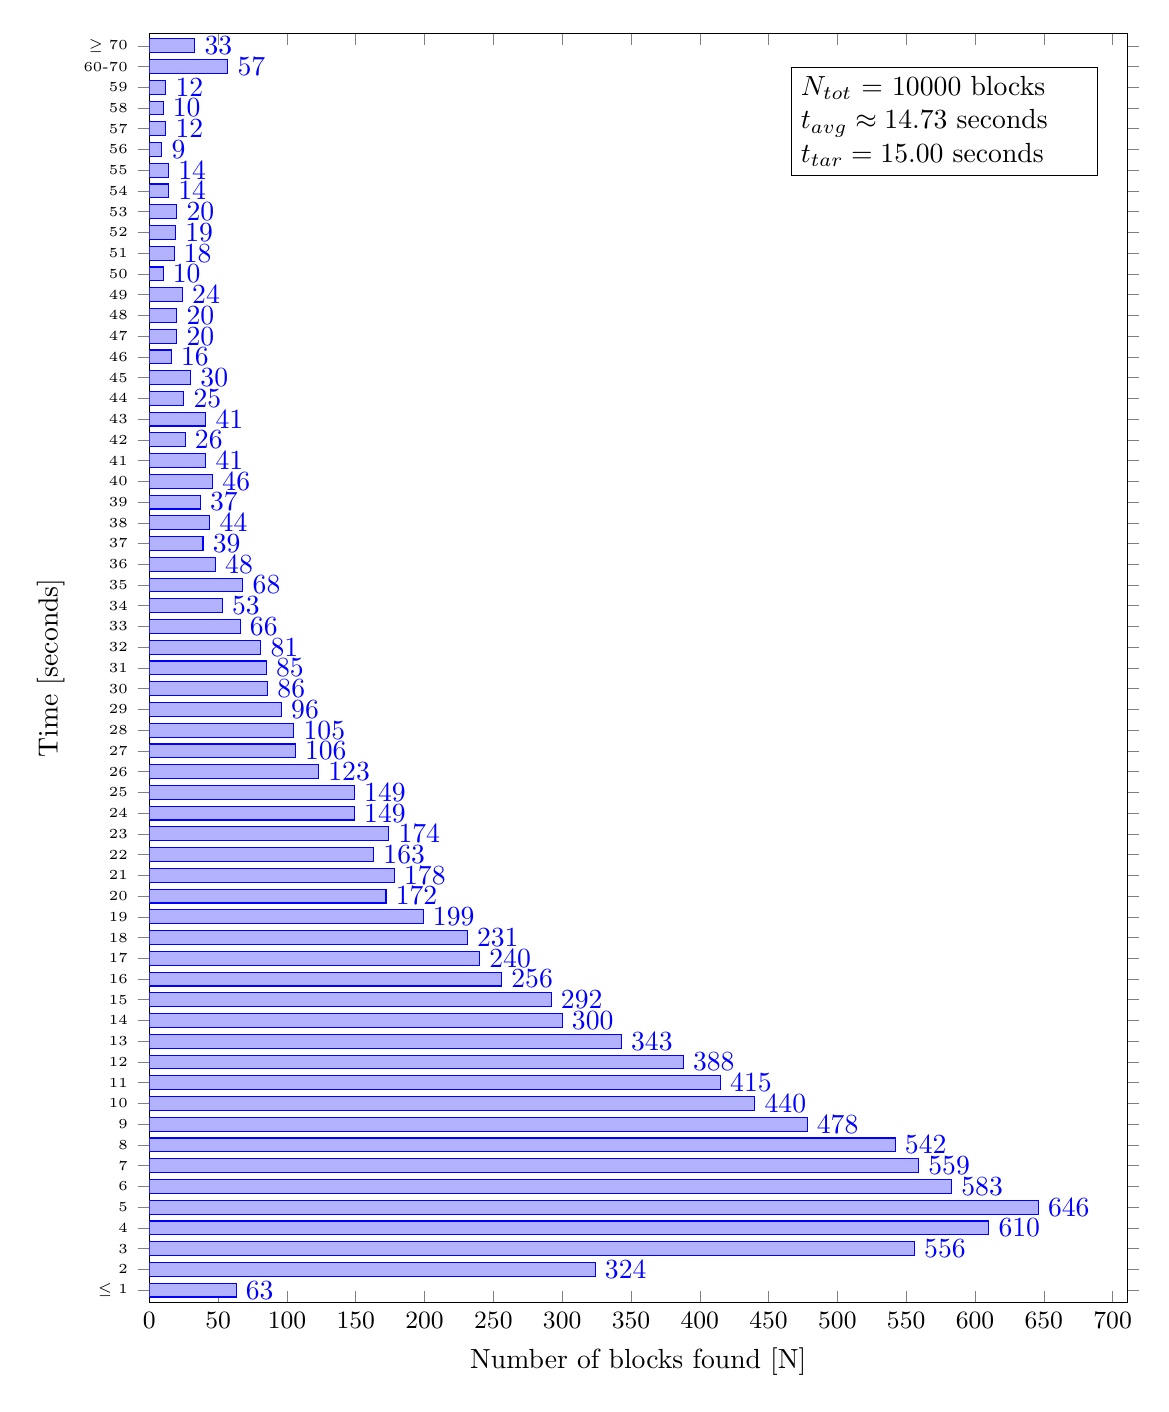
\begin{tikzpicture}
\node[draw, text width=3.65cm] at (10.1,15.0) 
    {$N_{tot}$ = 10000 blocks\\
    $t_{avg} \approx 14.73$ seconds\\
    $t_{tar} = 15.00$ seconds};
\begin{axis}[xbar,xmin=0,width=14cm, height=17.7cm, bar width=5pt,enlarge y limits=0.01,
y tick label style={font=\tiny},
x tick label style={font=\small},
xlabel={Number of blocks found [N]},
ylabel={Time [seconds]},
symbolic y coords={$\leq1$,2,3,4,5,6,7,8,9,10,11,12,13,14,15,16,17,18,19,20,21,22,23,24,25,26,27,28,29,30,31,32,33,34,35,36,37,38,39,40,41,42,43,44,45,46,47,48,49,50,51,52,53,54,55,56,57,58,59,60-70,$\geq70$},
ytick=data,
nodes near coords, nodes near coords align={horizontal},
]
\addplot coordinates {(63,$\leq1$) (324,2) (556,3) (610,4) (646,5) (583,6) (559,7) (542,8) (478,9) (440,10) (415,11) (388,12) (343,13) (300,14) (292,15) (256,16) (240,17) (231,18) (199,19) (172,20) (178,21) (163,22) (174,23) (149,24) (149,25) (123,26) (106,27) (105,28) (96,29) (86,30) (85,31) (81,32) (66,33) (53,34) (68,35) (48,36) (39,37) (44,38) (37,39) (46,40) (41,41) (26,42) (41,43) (25,44) (30,45) (16,46) (20,47) (20,48) (24,49) (10,50) (18,51) (19,52) (20,53) (14,54) (14,55) (9,56) (12,57) (10,58) (12,59) (57,60-70) (33,$\geq70$)};
\end{axis}
\end{tikzpicture}
\caption{Results of the Ethereum block time distribution test.}
\label{fig:ethtimetest}
\end{figure}

\pagebreak

\section{Visual representation of agreement states} \label{section:appendixdfa}

In Section \ref{section:statesofcontract}, a visual representation of the deterministic finite automaton $M$, which is shown in Figure \ref{fig:dfa}, was derived.

\begin{figure}[H]
\begin{center}
\begin{tikzpicture}[node distance=4cm,on grid,auto,initial text=, bend angle=25] 
   \node[state,initial,minimum size=5em] 		(CREATED)   							{{\tiny CREATED}}; 
   \node[state,minimum size=5em] 				(LOCKED)	[above right=of CREATED] 	{\tiny LOCKED};
   \node[state,accepting,minimum size=5em] 		(INACTIVE)	[below right=of CREATED] 	{\tiny INACTIVE};
   \node[state,minimum size=5em] 				(TRANSIT)	[below right=of LOCKED] 	{\tiny TRANSIT};
   \node[state,minimum size=5em] 				(TRANSITV)	[above right=of TRANSIT] 	{\tiny TRANSIT$_\mathrm{V}$};
   \node[state,minimum size=5em] 				(DELIV)		[below right=of TRANSIT] 	{\tiny DELIV};
   \node[state,minimum size=5em] 				(DELIVV)	[below right=of TRANSITV] 	{\tiny DELIV$_\mathrm{V}$};
   \node[state,accepting,minimum size=5em] 		(COMPLETED)	[below right=of INACTIVE] 	{\tiny COMPLETED};
   \node[state,minimum size=5em] 				(RETURNV)	[below right=of DELIV]	 	{\tiny RETURN$_\mathrm{V}$};
   \node[state,minimum size=5em] 				(RETURN)	[below right=of COMPLETED]	{\tiny RETURN};
   \node[state,minimum size=5em] 				(RETURNED)	[below left=of COMPLETED]	{\tiny RETURNED};
   \node[state,minimum size=5em] 				(RETURNEDV)	[below right=of RETURNED]	{\tiny RETURNED$_\mathrm{V}$};
   \node[state,minimum size=5em] 				(CLERKV)	[below left=of RETURNED]	{\tiny CLERK$_\mathrm{V}$};
   \node[state,minimum size=5em] 				(CLERK)		[below left=of INACTIVE]	{\tiny CLERK};
   
    \path[->] 
    (CREATED) 	edge [loop below] 		node[align=center,xshift=-11mm,yshift=12mm]					{$e_{\mathrm{prop}}$ \\ $e_{\mathrm{b\_abort}}$ \\ $ e_{\mathrm{decline}}$} 	()
    (CREATED) 	edge [bend left] 		node[align=center]											{$e_{\mathrm{accept}}$} 										(LOCKED)
    (CREATED) 	edge [bend right] 		node[align=center]											{$e_{\mathrm{s\_abort}}$} 									(INACTIVE)
    (LOCKED) 	edge			 		node[align=center]											{$e_{\mathrm{b\_abort}}$ \\ $e_{\mathrm{s\_abort}}$} 					(INACTIVE)
    (LOCKED) 	edge [bend left] 		node[align=center]											{$e_{\mathrm{s\_post}}$} 									(TRANSIT)
    (TRANSIT) 	edge [bend left] 		node[align=center,swap]										{$e_{\mathrm{viol}}$} 										(TRANSITV)
    (TRANSIT) 	edge [bend right] 		node[align=center]											{$e_{\mathrm{b\_deliver}}$} 									(DELIV)
    (TRANSITV) 	edge [loop below] 		node[align=center]											{$e_{\mathrm{viol}}$}										()
    (TRANSITV) 	edge [bend left] 		node[align=center]											{$e_{\mathrm{b\_deliver}}$}									(DELIVV)
    (DELIV) 	edge [bend right] 		node[align=center,swap]										{$e_{\mathrm{b\_nofeed}}$ \\ $e_{\mathrm{b\_approve}}$}				(COMPLETED)
    (DELIV) 	edge [bend right=20]	node[align=center,swap,near end,xshift=1mm]					{$e_{\mathrm{b\_reject}}$}									(RETURN)
    (DELIVV) 	edge [bend left=30] 	node[align=center,near start,swap,xshift=3mm,yshift=6mm]						{$e_{\mathrm{b\_nofeed}}$ \\ $e_{\mathrm{b\_approve}}$}				(COMPLETED)
    (DELIVV) 	edge [bend left=10] 	node[align=center,near end,swap,yshift=-4mm]				{$e_{\mathrm{b\_reject}}$}									(RETURNV)
    (RETURN) 	edge [bend right=15]		node[align=center]										{$e_{\mathrm{viol}}$}										(RETURNV)
    (RETURN) 	edge [bend left=20]		node[align=center,xshift=8mm]							{$e_{\mathrm{s\_deliver}}$}									(RETURNED)
    (RETURNV) 	edge [bend left=40]		node[align=center]											{$e_{\mathrm{s\_deliver}}$}									(RETURNEDV)
    (RETURNV) 	edge [loop left] 		node[align=center,xshift=10mm,yshift=6mm]					{$e_{\mathrm{viol}}$} 										()
    (RETURNED) 	edge [bend left]		node[align=center,near end]									{$e_{\mathrm{s\_reject}}$}									(CLERK)
    (RETURNED) 	edge					node[align=center,swap,near start]							{$e_{\mathrm{s\_nofeed}}$ \\ $e_{\mathrm{s\_approve}}$}				(INACTIVE)
    (RETURNEDV) edge [bend left=10]		node[align=center,swap]										{$e_{\mathrm{s\_reject}}$}									(CLERKV)
    (RETURNEDV) edge [bend right=10]	node[align=center,swap,xshift=2mm,yshift=-12mm]	{$e_{\mathrm{s\_nofeed}}$ \\ $e_{\mathrm{s\_approve}}$}	(INACTIVE)
    (CLERKV) 	edge [bend left=10]		node[align=center,near start,anchor=north west,xshift=-1mm,yshift=-5mm]	{$e_{\mathrm{clerk}}$}							(INACTIVE)
    (CLERK) 	edge [bend left]		node[align=center,near start]								{$e_{\mathrm{clerk}}$}										(INACTIVE);
\end{tikzpicture}
\caption{Visual representation of the deterministic finite automaton $M$.}
\label{fig:dfa}
\end{center}
\end{figure}